\documentclass{tietreport}
\let\cleardoublepage\clearpage
\hypersetup{hidelinks}
\usepackage{graphicx}
\usepackage{float}
\usepackage{booktabs}
\usepackage{array}
\usepackage{amsmath}
\usepackage{enumitem}
\usepackage{tikz}
\usetikzlibrary{arrows.meta, positioning}
\usepackage[
  date=year, style=alphabetic, backend=biber, sorting=nty,
  maxnames=5, minnames=3, maxalphanames=4, minalphanames=3,
  backref=true, doi=false, isbn=false, url=true, eprint=false
]{biblatex}
\addbibresource{references.bib}

\TitlePageHeader{UCS503 -- Software Engineering}
\ProjectTitle{Thapar Exchange}
\ProjectSubTitle{Campus Marketplace and Resource Sharing Platform}
\author{%
  \texttt{1024031005} Kanishk Khinchi \\
  \texttt{1024030290} Mahesh \\
  \texttt{1024030729} Amrita%
}
\TitlePageSubText{Group: 3C53, BE Third Year, C0E}
\AdvisorName{Dr. Paramveer Sidhu}
\TitlePageFooterText{{%
  \large Project Evaluation Report \\[0.2cm]
  \bfseries Computer Science and Engineering Department%
  } \\[0.15cm]
  Thapar Institute of Engineering and Technology, Patiala%
}

\begin{document}
\maketitle
\tableofcontents

\chapter{Introduction}
\section{Background and Context}
Students often need resources for a limited period, including textbooks, calculators, cycles, sports equipment, electronics, hostel essentials, and other useful items. Buying every item new can be expensive and unnecessary when a resource is needed temporarily. At the same time, students may own items that are no longer in regular use but could be useful to others.

Such exchanges are often arranged through messaging groups, personal contacts, or informal social media posts. These approaches can make it difficult to discover relevant items, compare details, confirm availability, and maintain a structured record of rental requests. Thapar Exchange, also referred to as ThaparRent in the repository README, is a campus-focused web application intended to make student-to-student resource sharing more organized.

The repository contains a React-based frontend and an Express backend connected to a PostgreSQL database through Prisma ORM. The current backend includes account registration and login, listing endpoints, and rental-booking workflows. The project is under active development; therefore, this report distinguishes implemented functionality from broader features proposed for future versions.

\subsection{Problem Statement}
Students at Thapar Institute of Engineering and Technology may need to rent or share items, but informal channels do not provide a single structured place to publish listings, browse resources, authenticate users, and manage rental requests. Information can be scattered across different groups, while requests and their statuses may be difficult to track consistently.

The project addresses this problem through a web-based campus marketplace with user accounts, item listings, and a database-backed booking process. The current backend supports registration and login, public listing retrieval, authenticated listing creation, and booking requests with owner-controlled acceptance or rejection. Institutional email verification, advanced search filters, condition documentation, reporting, and administrative moderation should not be considered complete unless verified in the current code.

\section{Project Objectives}
\begin{enumerate}[label=\arabic*.]
  \item Develop a centralized web application for students to discover and offer campus resources.
  \item Implement registration and login, storing password hashes rather than plaintext passwords.
  \item Provide listing endpoints for item details, category, daily rental price, optional image URL, availability, and owner.
  \item Implement rental requests and owner-controlled acceptance or rejection.
  \item Store users, listings, and bookings in PostgreSQL using Prisma ORM.
  \item Validate core workflows and document limitations before making performance, usability, or security claims.
\end{enumerate}

\section{Scope and Limitations}
This report focuses on the repository's architecture, backend modules, data model, and local database setup. The observed setup results are that Prisma schema validation succeeded, Prisma Client was generated, and the existing initialization and booking migrations were applied successfully to the local PostgreSQL database. This does not independently establish that every end-to-end user workflow works.

No verified performance benchmarks, formal usability-study results, or evidence that all planned trust and moderation features are complete were supplied. These are treated as evaluation tasks or future work rather than implemented outcomes.

\chapter{Methodology and Design}
\section{System Architecture}
The application follows a client--server architecture. The frontend uses React and Vite \cite{reactdocs,vitedocs}. It communicates with a backend API implemented using Node.js and Express \cite{expressdocs}. The backend uses Prisma ORM to access a PostgreSQL database \cite{prismadocs,postgresdocs}. During local development, the Vite configuration proxies API requests to the backend.

Figure~\ref{fig:system-architecture} presents the high-level component arrangement. Requests originate in the browser-based frontend, are handled by Express routes and middleware, and access persistent data through Prisma.

\begin{figure}[H]
\centering
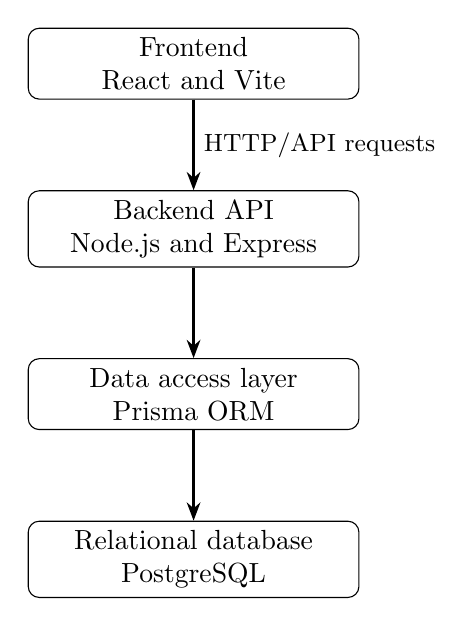
\begin{tikzpicture}[
  node distance=1.15cm,
  component/.style={draw, rounded corners, align=center, minimum width=4.2cm, minimum height=0.9cm},
  connection/.style={-{Stealth}, thick}
]
\node[component] (frontend) {Frontend\\React and Vite};
\node[component, below=of frontend] (backend) {Backend API\\Node.js and Express};
\node[component, below=of backend] (orm) {Data access layer\\Prisma ORM};
\node[component, below=of orm] (database) {Relational database\\PostgreSQL};
\draw[connection] (frontend) -- node[right, font=\small]{HTTP/API requests} (backend);
\draw[connection] (backend) -- (orm);
\draw[connection] (orm) -- (database);
\end{tikzpicture}
\caption{High-level architecture of Thapar Exchange}
\label{fig:system-architecture}
\end{figure}

The main entities are users, listings, and bookings. A user can own multiple listings, and a listing can have multiple booking records. Each booking identifies a listing and a renter, and stores a status and timestamps. Listing states are \texttt{AVAILABLE} and \texttt{UNAVAILABLE}; booking states are \texttt{PENDING}, \texttt{ACCEPTED}, \texttt{REJECTED}, and \texttt{CANCELLED}.

\subsection{High-Level Workflow}
\begin{enumerate}
  \item A student registers using a name, email address, and password, or logs in with existing credentials.
  \item The backend validates the request, hashes new passwords with bcrypt \cite{bcrypt}, and issues a JSON Web Token (JWT) after successful authentication \cite{jwt}.
  \item Public listing endpoints allow clients to retrieve listings and listing details.
  \item An authenticated student creates a listing. The backend derives the owner identity from the authentication token rather than trusting an owner ID supplied in the request body.
  \item A renter submits a booking request for an available listing. The backend prevents a user from requesting their own listing and rejects duplicate pending requests for the same listing by the same renter.
  \item The listing owner can accept or reject a pending booking. The booking status is persisted in the database.
\end{enumerate}

\subsection{Technical Stack}
\begin{table}[H]
\centering
\caption{Technologies used in the current repository}
\begin{tabular}{p{0.28\textwidth} p{0.62\textwidth}}
\toprule
\textbf{Technology} & \textbf{Role in the project}\\
\midrule
JavaScript & Main language used by the frontend and backend.\\
React & Browser-based user interface.\\
Vite & Development server and frontend build tooling.\\
Node.js & Runtime for the backend API.\\
Express 5 & HTTP routes and middleware.\\
PostgreSQL & Relational database for users, listings, and bookings.\\
Prisma ORM & Database schema, client access, and migrations.\\
bcrypt & Password hashing.\\
JSON Web Token (JWT) & Authentication tokens for protected API requests.\\
Git & Version control for source files and project history.\\
\bottomrule
\end{tabular}
\end{table}

\section{Implementation Details}
\subsection{Authentication and Listing Management}
The authentication routes are implemented in \texttt{backend/src/auth.routes.js}. Registration accepts a name, email, and password. The backend hashes the password using bcrypt and stores the hash in the user record. Login checks submitted credentials and returns a JWT and public user information. The middleware in \texttt{backend/src/auth.middleware.js} protects routes that require authentication.

Listing functionality is implemented in \texttt{backend/src/listings.routes.js}. The database schema defines title, description, category, daily price, optional image URL, status, owner ID, and timestamps. Listing retrieval endpoints are public, while listing creation requires authentication. The owner ID is derived from the authenticated user, helping prevent clients from creating listings on behalf of another account.

\subsection{Rental Booking Workflow}
Booking functionality is implemented in \texttt{backend/src/bookings.routes.js}. An authenticated renter can request an available listing. The renter identity is derived from the token, and a user cannot request their own listing. The backend also rejects a duplicate pending request by the same renter for the same listing.

A listing owner can retrieve booking requests associated with their listings and change a pending booking to \texttt{ACCEPTED} or \texttt{REJECTED}. These controls provide a basic structured rental-request workflow; they do not establish that physical handover, item-condition verification, payment, dispute resolution, or return confirmation has been implemented.

\subsection{Database Design}
The Prisma schema defines three main models:
\begin{itemize}
  \item \textbf{User:} Unique email address, name, password hash, related listings, related bookings, and timestamps.
  \item \textbf{Listing:} Item details, daily price, optional image URL, availability status, owner relationship, and timestamps.
  \item \textbf{Booking:} Listing and renter relationships, request status, and timestamps. Indexes support queries by listing/status and renter/creation time.
\end{itemize}

Figure~\ref{fig:er-model} presents a conceptual view of the entities and relationships. Exact fields and constraints are defined by the repository's Prisma schema.

\begin{figure}[H]
\centering
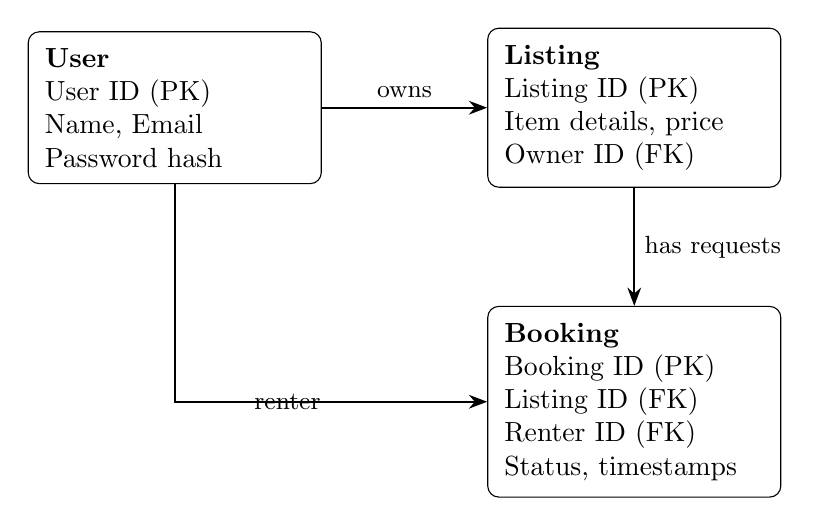
\begin{tikzpicture}[
  node distance=2.1cm,
  entity/.style={draw, rounded corners, align=left, text width=3.3cm, minimum height=1.8cm, inner sep=6pt},
  relation/.style={-{Stealth}, thick}
]
\node[entity] (user) {\textbf{User}\\User ID (PK)\\Name, Email\\Password hash};
\node[entity, right=of user] (listing) {\textbf{Listing}\\Listing ID (PK)\\Item details, price\\Owner ID (FK)};
\node[entity, below=1.5cm of listing] (booking) {\textbf{Booking}\\Booking ID (PK)\\Listing ID (FK)\\Renter ID (FK)\\Status, timestamps};
\draw[relation] (user) -- node[above, font=\small]{owns} (listing);
\draw[relation] (listing) -- node[right, font=\small]{has requests} (booking);
\draw[relation] (user.south) |- node[pos=0.75, left, font=\small]{renter} (booking.west);
\end{tikzpicture}
\caption{Conceptual entity--relationship model}
\label{fig:er-model}
\end{figure}

The backend README documents configuration through a \texttt{DATABASE\_URL} connection string and a private \texttt{JWT\_SECRET}. Credentials should be stored in a local environment file and must not be committed to the repository. Database migrations and Prisma Client generation must run against a correctly configured PostgreSQL instance.

\chapter{Results and Evaluation}
\section{Environment and Database Setup}
The local database setup was performed using PostgreSQL and Prisma. The following outcomes were observed in the development terminal:
\begin{itemize}
  \item Prisma schema validation completed successfully.
  \item Prisma Client generation completed successfully.
  \item The existing initialization migration and booking-related migration were applied.
  \item Prisma reported that the database was in sync with the schema.
\end{itemize}
These outcomes verify database configuration and migration execution in the local development environment. They do not prove that all API endpoints or frontend workflows have passed functional testing.

\section{Functional Test Plan}
The following test cases should be executed and their observed results recorded before they can be marked as passed.

\begin{table}[H]
\centering
\caption{Functional test cases and expected outcomes}
\small
\begin{tabular}{p{0.18\textwidth} p{0.43\textwidth} p{0.29\textwidth}}
\toprule
\textbf{Test area} & \textbf{Test case} & \textbf{Expected outcome}\\
\midrule
Database & Validate schema and apply migrations & Schema valid; migrations applied\\
Authentication & Register with valid details & Account created and password hashed\\
Authentication & Login with incorrect credentials & Request rejected\\
Authentication & Access protected route without token & Request rejected\\
Listings & Retrieve public listings & Listing data returned\\
Listings & Create listing without authentication & Request rejected\\
Bookings & Request own listing & Request rejected\\
Bookings & Submit duplicate pending request & Duplicate request rejected\\
Bookings & Owner updates pending request & Status changes to accepted or rejected\\
Integration & Retrieve records after create/update & Persisted state is returned\\
Frontend & Use UI while backend is running & UI handles success/error states\\
\bottomrule
\end{tabular}
\end{table}

The database setup cases above were observed as successful. The remaining functional cases are test recommendations until their execution and results are recorded. No unsupported pass rate is reported.

\section{Performance Evaluation}
The available repository and terminal output do not provide verified measurements of API response time, throughput, concurrent-user capacity, or user-study outcomes. Numerical performance claims are therefore not made. Future evaluation should record:
\begin{itemize}
  \item \textbf{API response time:} Median and 95th-percentile response times under a documented workload.
  \item \textbf{Authentication correctness:} Successful and rejected registration/login cases.
  \item \textbf{Listing workflow correctness:} Whether valid operations succeed and invalid requests are rejected.
  \item \textbf{Booking workflow correctness:} Ownership, availability, duplicate pending requests, and status transitions.
  \item \textbf{Database consistency:} Related records after create and update operations.
  \item \textbf{Usability feedback:} Student completion of listing discovery and booking tasks, with feedback recorded.
\end{itemize}

\section{Analysis}
The repository establishes a backend foundation for a campus rental platform. It includes authentication, protected listing creation, public listing retrieval, booking requests, ownership checks, status transitions, and a relational data model. The separate frontend, API server, and database layer provide a modular structure for further development.

Features such as richer search and filtering, institutional student verification, condition documentation, reporting, and administrative moderation should not be treated as complete unless confirmed in the current code and tested in the running application. The available source and migration output do not provide measured evidence of system performance or student acceptance. A complete evaluation requires repeatable API tests, frontend integration checks, and feedback from target users.

\section{Limitations}
\begin{itemize}
  \item Only schema validation, client generation, and migration execution are confirmed by the available terminal output.
  \item Functional API and end-to-end frontend tests have not been documented here as completed.
  \item No performance benchmark, load test, or usability study has been supplied.
  \item Institutional verification, moderation, condition records, payments, and dispute management require separate implementation and verification where applicable.
  \item Successful local setup does not establish production readiness; deployment, secret management, logging, validation, authorization, and security controls need further review.
\end{itemize}

\chapter{Conclusion}
\section{Summary of Work}
Thapar Exchange is a campus marketplace and resource-sharing project intended to help students discover and offer useful items through a structured web platform. The repository contains a React frontend, a Node.js and Express backend, and a PostgreSQL database accessed through Prisma ORM. The backend supports account registration and login, listing retrieval and creation, and a rental booking workflow with owner-controlled acceptance or rejection.

The local database setup was completed successfully: the schema validated, the Prisma Client was generated, and the existing migrations were applied. The next step is to test the application end to end so that the working status of each user-facing workflow can be documented accurately.

\section{Key Findings}
\begin{itemize}
  \item The repository uses a modular client--server architecture with a relational database layer.
  \item Password hashing and JWT-based authentication are used in the backend authentication flow.
  \item Listing and booking routes include ownership and request-state checks, including prevention of duplicate pending requests.
  \item Database schema validation, client generation, and migration execution succeeded in the local environment.
  \item Broader trust, moderation, and condition-documentation features require verification before being described as complete.
  \item Numerical performance claims should be added only after documented measurements have been collected.
\end{itemize}

\section{Future Work and Recommendations}
\begin{enumerate}
  \item Complete and validate frontend workflows for registration, login, listing creation, listing discovery, and booking management.
  \item Implement and verify institutional email validation if access should be restricted to eligible TIET students.
  \item Add search and filtering by category, price, availability, and pickup location where not already implemented.
  \item Introduce item-condition documentation and reporting mechanisms to improve transparency and trust.
  \item Develop moderation and administration tools for reported listings and inappropriate content.
  \item Add automated tests for authentication, listing permissions, booking status transitions, and database consistency.
  \item Conduct usability testing with students and benchmark API response times under a documented workload.
  \item Review deployment configuration, secret management, input validation, logging, and access control before real-world launch.
\end{enumerate}

\section{Final Remarks}
Thapar Exchange addresses a practical campus need: making it easier for students to find and share resources. The current repository provides core backend building blocks for users, listings, and rental requests, together with a modern web development stack. The next stage should focus on verifying end-to-end functionality, completing important trust and usability features, and collecting documented test evidence. The project should be presented as an evolving academic software system, with implemented capabilities and future plans clearly distinguished.

\printbibliography[heading=bibintoc]
\end{document}